\chapter{Overall description}
\labch{options}
	\section{Product perspective}
		\subsection{Scenarios}
			\textbf{Student signs up to S\&C}
			\begin{flushleft}
				Student Bob enters in the system for the first time. On the homepage, he first clicks the \emph{Registration button} and then the \emph{Student Registration button}. To register, Bob fills out a form providing its institutional e-mail (bob.johnson@mail.polimi.it) and password (which will be used for future logins), a brief description of his academic background and specifies whether he would like to take part to the recommendation analysis. Finally, Bob uploads his CV by clicking the \emph{Upload CV button}. Now Bob is registered and can search for internships that interest him.
			\end{flushleft}
			\textbf{Company signs up to S\&C}
			\begin{flushleft}
				The company FinestraMI enters the system for the first time. On the homepage, it first clicks the \emph{Registration button} and then the \emph{Company Registration button}. To register, the company fills out a form providing its name, a brief description of its area of expertise and its business area (the market where it operates) and finally its corporate e-mail (info@finestrami.it) and password (which will be used for future logins). FinestraMI also specifies, by selecting the appropriate option, whether it wants take part into the recommendation analysis. Now, FinestraMI is registered and can publish its internships advice.
			\end{flushleft}
			\textbf{Company publishes an internship offer}
			\begin{flushleft}
				The company FinestraMI enters in the system; on the homepage, it clicks the \emph{Login button}. Once logged in, FinestraMI accesses the \emph{Publish New Internship section}. A new internship advice is added by filling out a form where the following information is provided:
				\begin{itemize}
					\item "Window restore" (the intership title);
					\item "The aim of this internship is to give to student to opportunity to repair office windows and..." (a brief description);
					\item "third year bachelor students..." (experience required);
					\item "not suffering from dizziness" (desired skills);
					\item "1. coordination of glass disposal; 2. ..." (main activities the internship involves);
					\item "no paid, canteen tickets available" (terms of the internship);
					\item "22/11/2024" (advice deadline).
				\end{itemize}
				
				Now the internship advice is visible to students registered on the platform (and also to FinestraMI).
			\end{flushleft}
			\textbf{Student proactively searches for an internship}
			\begin{flushleft}
				Students Bob, Alice and Micheal access to the system by clicking "Login". Each one of them wants to find an internship to apply but each one of them has a different idea of what and where he/she would like to do/be:
				\begin{itemize}
					\item Bob is really interested on doing practice on an handwork but he neither knows a name of a company nor knows which kind of handwork apply for so, he goes to the \emph{View Internships section}, where he can see all the published internships, listed from the most recent to the least recent. The most recent one is "Window restore" by FinestraMI, then he selects it;
					\item Alice has not already decided the kind of internship she wants to apply for but knows many names of companies that operate near her home and so she prefers to go to the \emph{View Companies section}, where she can see all the registered companies and all the internships published by each company. Then she recognized FinestraMI and since she knows that it is expanding, she decides to select it. "Window restore" is the only available advice of FinestraMI but she select it anyways;
					\item Micheal is looking forward to do an internship related to windows restoration, so he uses the search bar to insert "windows restoration" and selects the option "only paid internships", but no internship are found. Then he removes the option and find the internship of FinestraMI. Since it is the only left, he selects it.
				\end{itemize} 
			\end{flushleft}
			\textbf{Student receive a notification about a new internship}
			\begin{flushleft}
				The company CancellaMI (previously registered to the platform) publishes a new internship related to railings maintenance then, Student Bob, who has chosen to be notified by the system when new internships that might be of interest are published, receives an email informing it that a new intership related to his studies is available, since it stated in his CV that after the internship at FinestraMI he became passionate of railings. Bob then logs into the platform and, by going to the \emph{Notification section}, can view the internships offer in more detail.
			\end{flushleft}
			\textbf{Company receives a notification about new possibly interested students}
			\begin{flushleft}
				Company FinestraMI, which has chosen to be notified by the system, receives an email informing it that new students are appealing for its intership "Window Restore" (based on their CVs). FinestraMI then logs into the platform, goes into the \emph{Internship section}, clicks on \emph{Windows restore internship} and by going to the \emph{Notification section} can view the students'profiles and their CVs in more detail.
			\end{flushleft}
			\textbf{Student applies for an internship}
			\begin{flushleft}
				Student Bob wants to apply for the internship "Windows restore". To do so, they log into the system, access the page for "Windows restore" internship and click the \emph{Apply button}. Automatically, the system will send a notification to FinestraMI (the company offering the internship) to inform it that Bob has applied
			\end{flushleft}
			\textbf{The company accepts the application of a student}
			\begin{flushleft}
				Company FinestraMI receives the email regarding student Bob's application for the internship "Window Restore". FinestraMI then logs into the platform, navigates to the \emph{Internships section}, select the \emph{Window Restore Internship}, goes to the \emph{Notification section} and clicks the \emph{Accept Application button} to approve Bob's application.
			\end{flushleft}
			\textbf{The company proposes to a student to apply for one of its internships}
			\begin{flushleft}
				contenuto...
			\end{flushleft}
			\textbf{Student accepts an internship proposal}
			\begin{flushleft}
				contenuto...
			\end{flushleft}
			\textbf{The application deadline expires and the selection process is configured}
			\begin{flushleft}
				The administrator of the company FinestraMI notices that the application deadline for the internship advice "Window Restore" (which was previously published on the platform) is now expired and selection process for that internship has not configured yet, so he goes to the designated page and configures:
				\begin{itemize}
					\item two steps (the selection process will be made up of two steps);
					\item a set of metrics to evaluate students ("manual skills" and "knowledge of materials" in this case);
					\item each step is configured as a questionnaire with a series of questions for the students, in this case in particular:
						\begin{enumerate}
							\item first step is test of both open and closed questions regarding knowledge of materials. For closed questions, the platform is also able to automatically check if they are corrected or not (and so, for each closed question, also the scores to assign to each possible answer are inserted into the system). Open questions will be evaluated manually by the company;
							\item second step is an oral exam. Since there are no predefined questions for this step, the company only inserts into the system one open question called "oral exam", scores will be inserted by the company at the end of the exam.
						\end{enumerate}
					\item for each step and for each candidate, the company chooses also the date in which it provides the questionnaire to the candidate.
				\end{itemize}
			\end{flushleft}
			\textbf{The selection process runs}
			\begin{flushleft}
				For the internship advice "Window restore", the company FinestraMI received three applications: Bob, Alice and Micheal. FinestraMI is planning to accept only one student at time, therefore it chooses to first call Micheal for the first step, since his curriculum impressed more the company. On \date{23/11/2024} Micheal is called and the questionnaire is given to him. His answers are evaluated (automatically for the closed ones and manually for the opened ones) and gets an overall score of 99 out of 100: the company decides to select him, discards Bob's application and leaves suspended the call for Alice. The company sets for Bob and Micheal the right message and the platform notifies them. 
			\end{flushleft}
			\textbf{User provides a feedback at the end of the selection process}
			\begin{flushleft}
				Micheal has just received the selection results for his application for the "Window restore" internship of FinestraMI. Attached to it, the system provides him an optional questionnaire where it asks to Micheal to evaluate his experience of the selection (questions are quite standard, such as "was the company on time with the interview appointments?", "did the questions related to the required skills" e.c.c.). Since it is not compulsory, Micheal does not compile it. On the other side, once the entire selection process of FinestraMI is closed, FinestraMI receives from the system a questionnaire to evaluate its experience (questions mainly concern the preparation level of the candidates, such as "was the number of students with the required skills below average?"). Then the company compiles it from the system.
			\end{flushleft}
			\textbf{User reports a complaint on one of the internship is currently doing}
			\begin{flushleft}
				Today, Alice who is currently enrolled in the internships at the company WeWorkGreat had a problem with the task that was given to her, she asks the helpdesk of the company where she is performing the internship and they ask her to upload a video on the company file sharing platform to show the situation. Alice notices that she can’t upload the video because the maximum uploading size for students is to 10 MB, then she opens Students\&Companies and writes a compliant that states that the file sharing system of WeWorkGreat is only of 10 MB.
			\end{flushleft}
			\textbf{User provides a feedback at the conclusion of an internship}
			\begin{flushleft}
				Alice has just finished the internship at WeWorkGreat, an non-compulsory questionnaire is given to her with some general questions related to her experience at the company (e.g. "did the company respect the terms listed in the advice?" e.c.c.). Since it is not compulsory, Alice decides to not compile it.
			\end{flushleft}
		\subsection{High-level class diagram}
			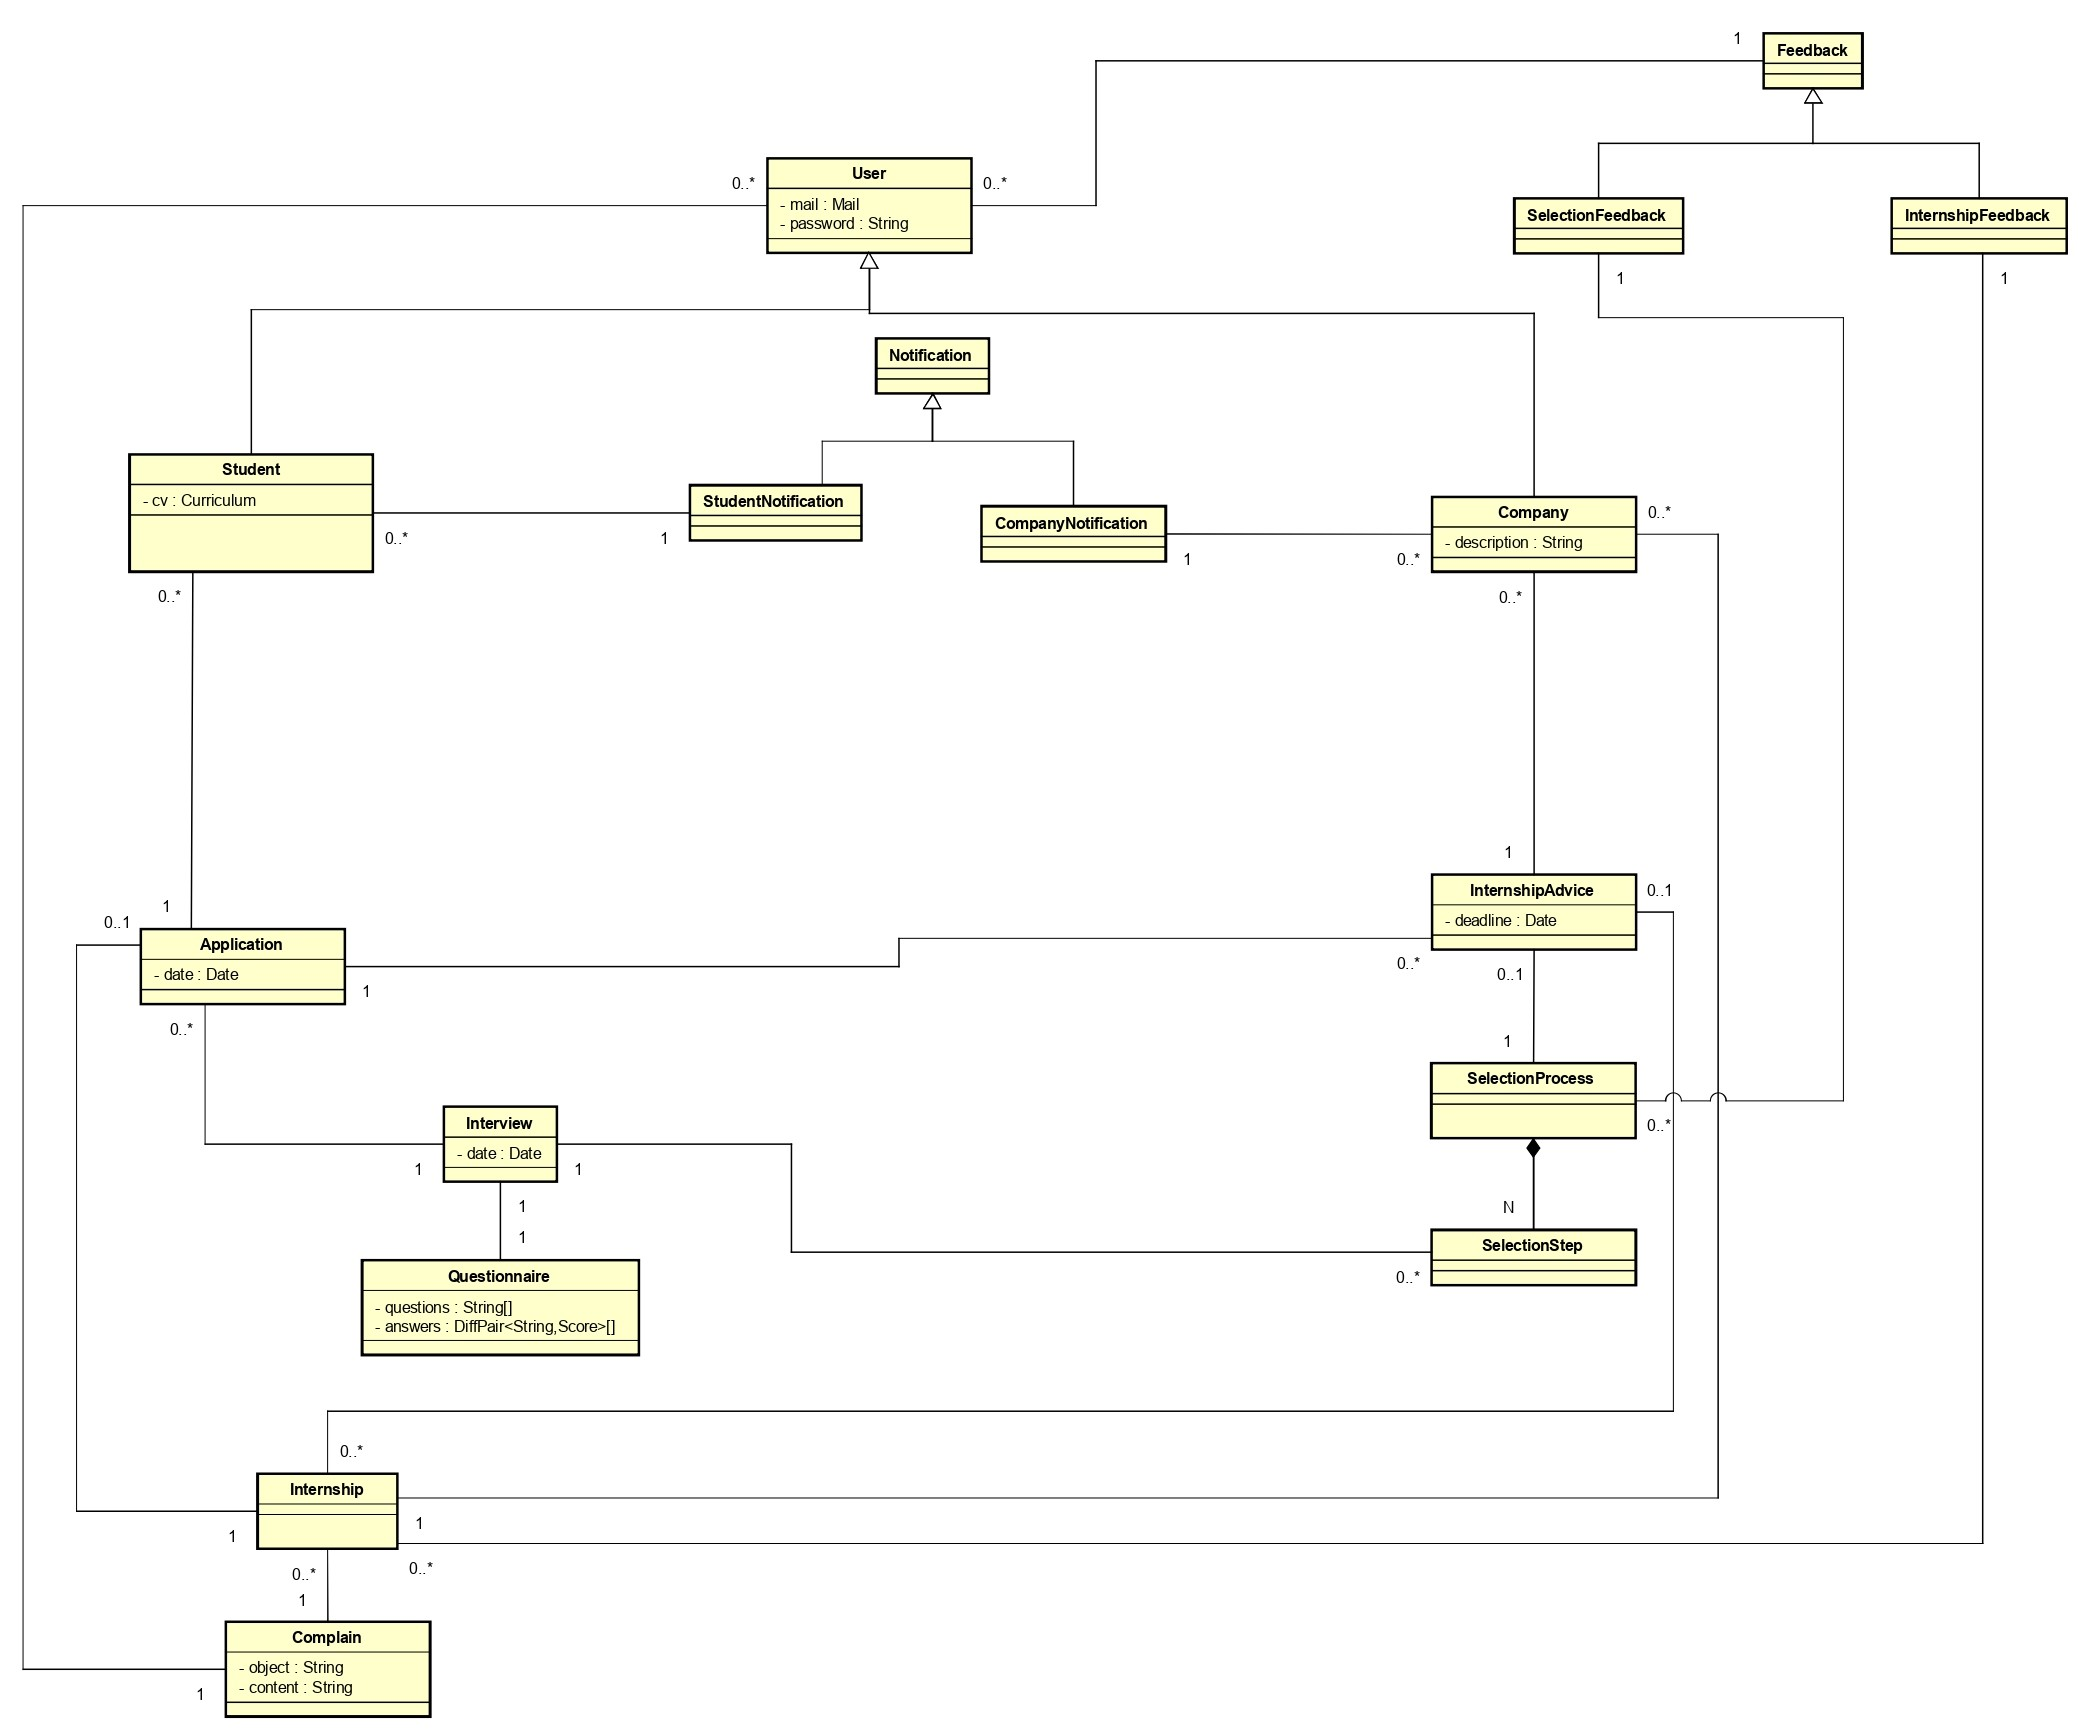
\includegraphics{class_diagram(NO NOT).jpg}
			
			This is the entire high-level class diagram. Due to the fact that it is quite large, perhaps it is convenient to divide it into four parts:
			\begin{itemize}
				\item \emph{application part}: \textsc{User} is specialized into \textsc{Company} (which publishes \textsc{InternshipAdvice}) and \textsc{Student} (which applies for \textsc{InternshipAdvice});
				\item \emph{selection part}: each \textsc{InternshipAdvice} is related to \textsc{SelectionProcess}, which is made up of a number of \textsc{SelectionStep}s that actualize in \textsc{Interviews}s for the students currently enrolled in the selection process;
				\item \emph{notification part}: both user categories may receive notifications, in particular (for simplicity they are not detailed into the diagram):
					\begin{itemize}
						\item \textsc{SelectionResultNotification}: notifies to a \textsc{Student} the result of a \textsc{SelectionProcess} it attended;
						\item \textsc{AdviceNotification}: notifies to a \textsc{Student} that an \textsc{InternshipAdvice} that might interests it has just been published;
						\item \textsc{InviteNotification}: notifies to a \textsc{Student} that a \textsc{Company} invited it to apply for one of its \textsc{InternshipAdvice};
						\item \textsc{InterestedStudentsNotification}: notifies to a \textsc{Company} a list of \textsc{Student}s that might be interested in applying to their \textsc{InternshipAdvice};
						\item \textsc{StudentAppNotification}: notifies to a \textsc{Company} that a \textsc{Student} applied for one of its \textsc{InternshipAdvice};
					\end{itemize}
				\item \emph{feedback\&complaints part}: \textsc{User}s can upload \textsc{Feedback}s and \textsc{Complaint}s.
			\end{itemize}
	\section{Product functions}
		\textbf{Sign-up and login}
			\begin{flushleft}
				contenuto...
			\end{flushleft}
		\textbf{Internship advice publication}
			\begin{flushleft}
				contenuto...
			\end{flushleft}
		\textbf{Internship application}
			\begin{flushleft}
				contenuto...
			\end{flushleft}
		\textbf{Internship candidates selection}
			\begin{flushleft}
				contenuto...
			\end{flushleft}
		\textbf{Candidates interview schedule}
			\begin{flushleft}
				contenuto...
			\end{flushleft}
		\textbf{Internship complaints}
			\begin{flushleft}
				contenuto...
			\end{flushleft}
	\section{User characteristics}
	\section{Assumptions, dependencies and constraints}